\documentclass[]{article}

\usepackage{graphicx}
\graphicspath{ {Images/} }
\usepackage{titlesec}
\usepackage{wrapfig}

\titleformat{\section}
  {\normalfont\Large\bfseries}{\thesection}{1em}{}[{\titlerule[0.8pt]}]

\begin{document}

\section*{IACS-Computes! 2016 Installing Anaconda}
Greetings Everyone, \\

For this camp, we will be using the Python distribution knows as Anaconda. Anaconda comes with a vast amount of libraries, Jupyter Notebooks with iPython, and has nice cross-platform support. Anaconda can be obtained for free from www.continuum.io, where the following instructions on installation can also be found (Just click on the downloads section). We will be using Python version 2.7 for this camp. We will be doing this as a group at the start of the camp.\\

Cheers, \\
 Bryan Sundahl
\vspace{1in}

\begin{centering}
    \centerline{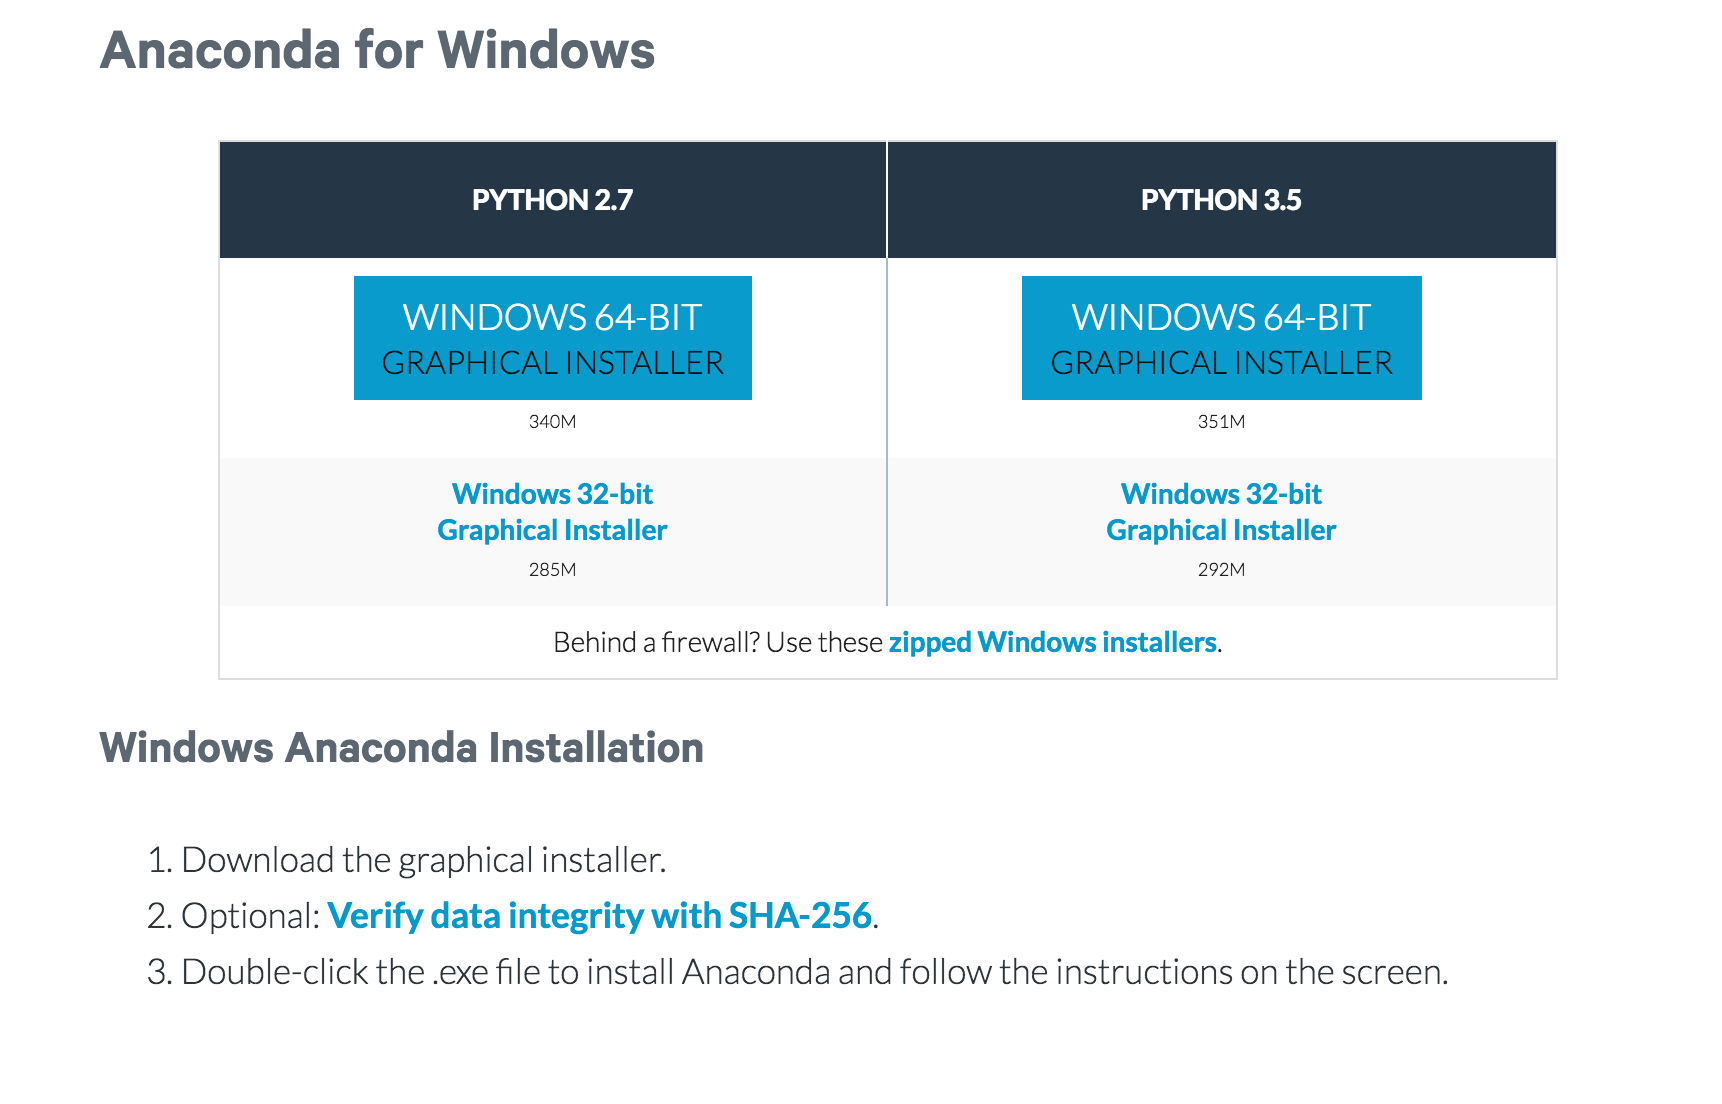
\includegraphics[scale=0.5]{windows.png}}
\end{centering}
\section*{IACS-Copmutes! 2016 Installing Anaconda}
\begin{centering}
    \centerline{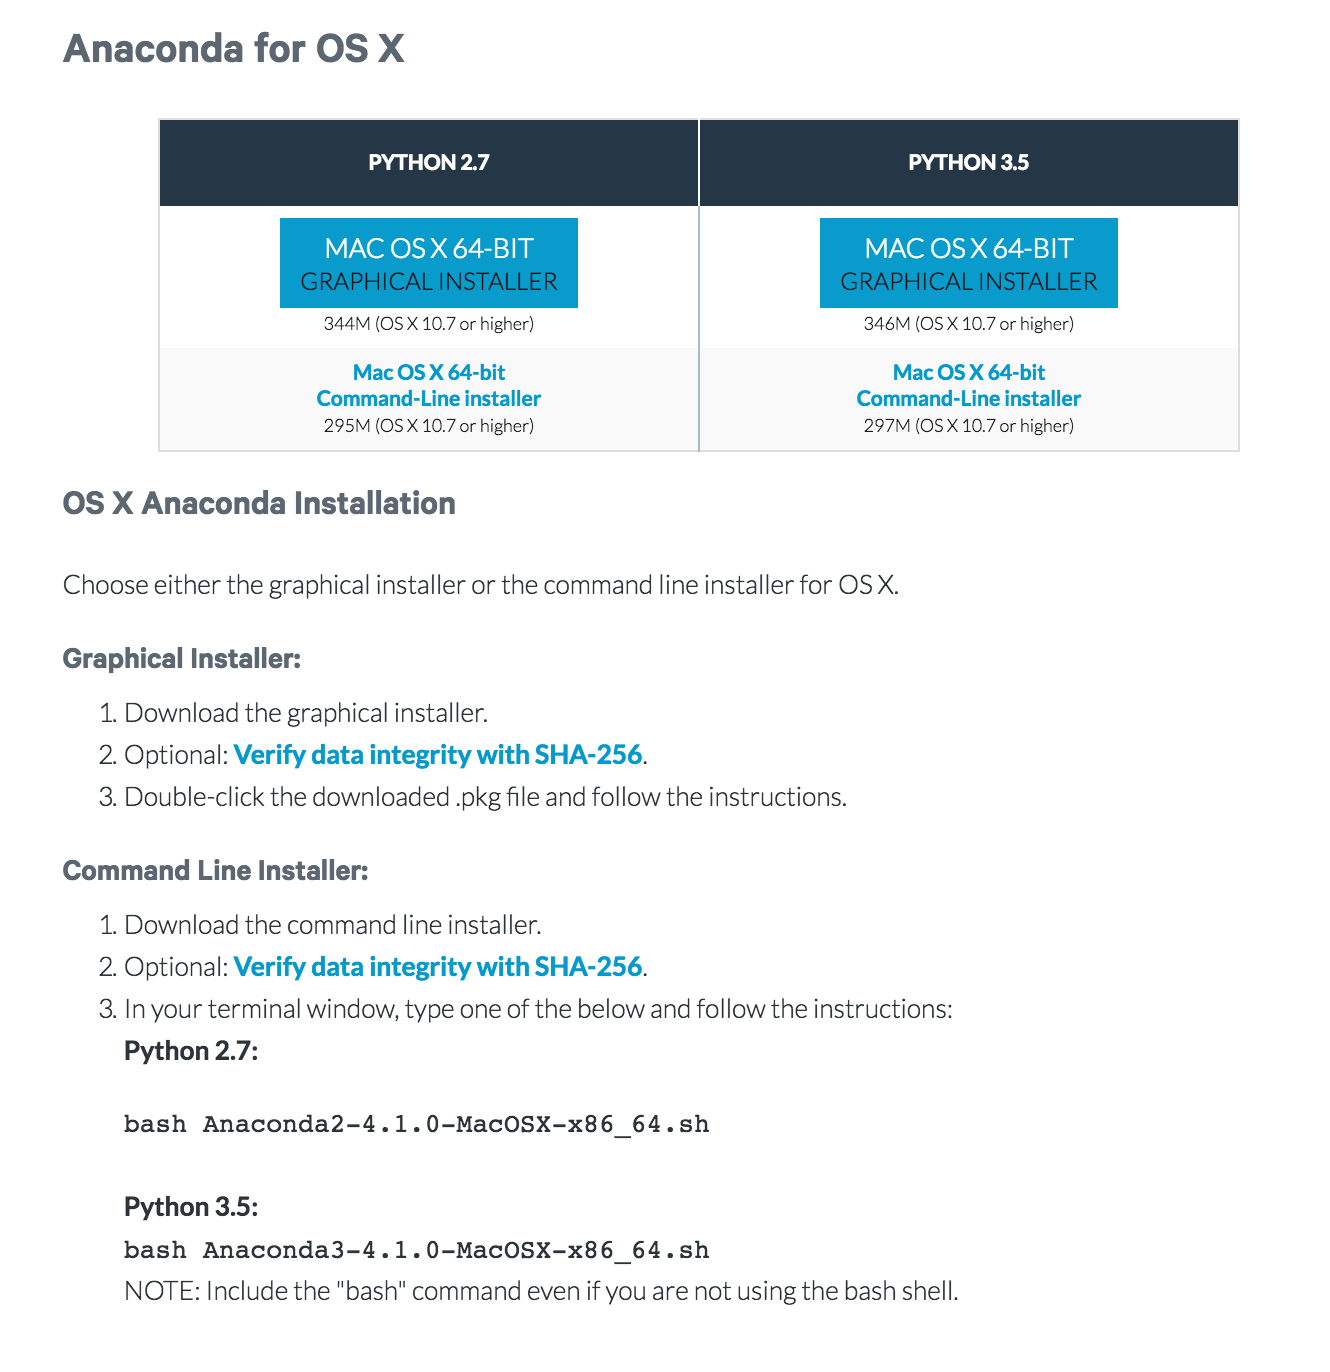
\includegraphics[scale=0.7]{mac.png}}
\end{centering}
\section*{IACS-Copmutes! 2016 Installing Anaconda}
\begin{centering}
    \centerline{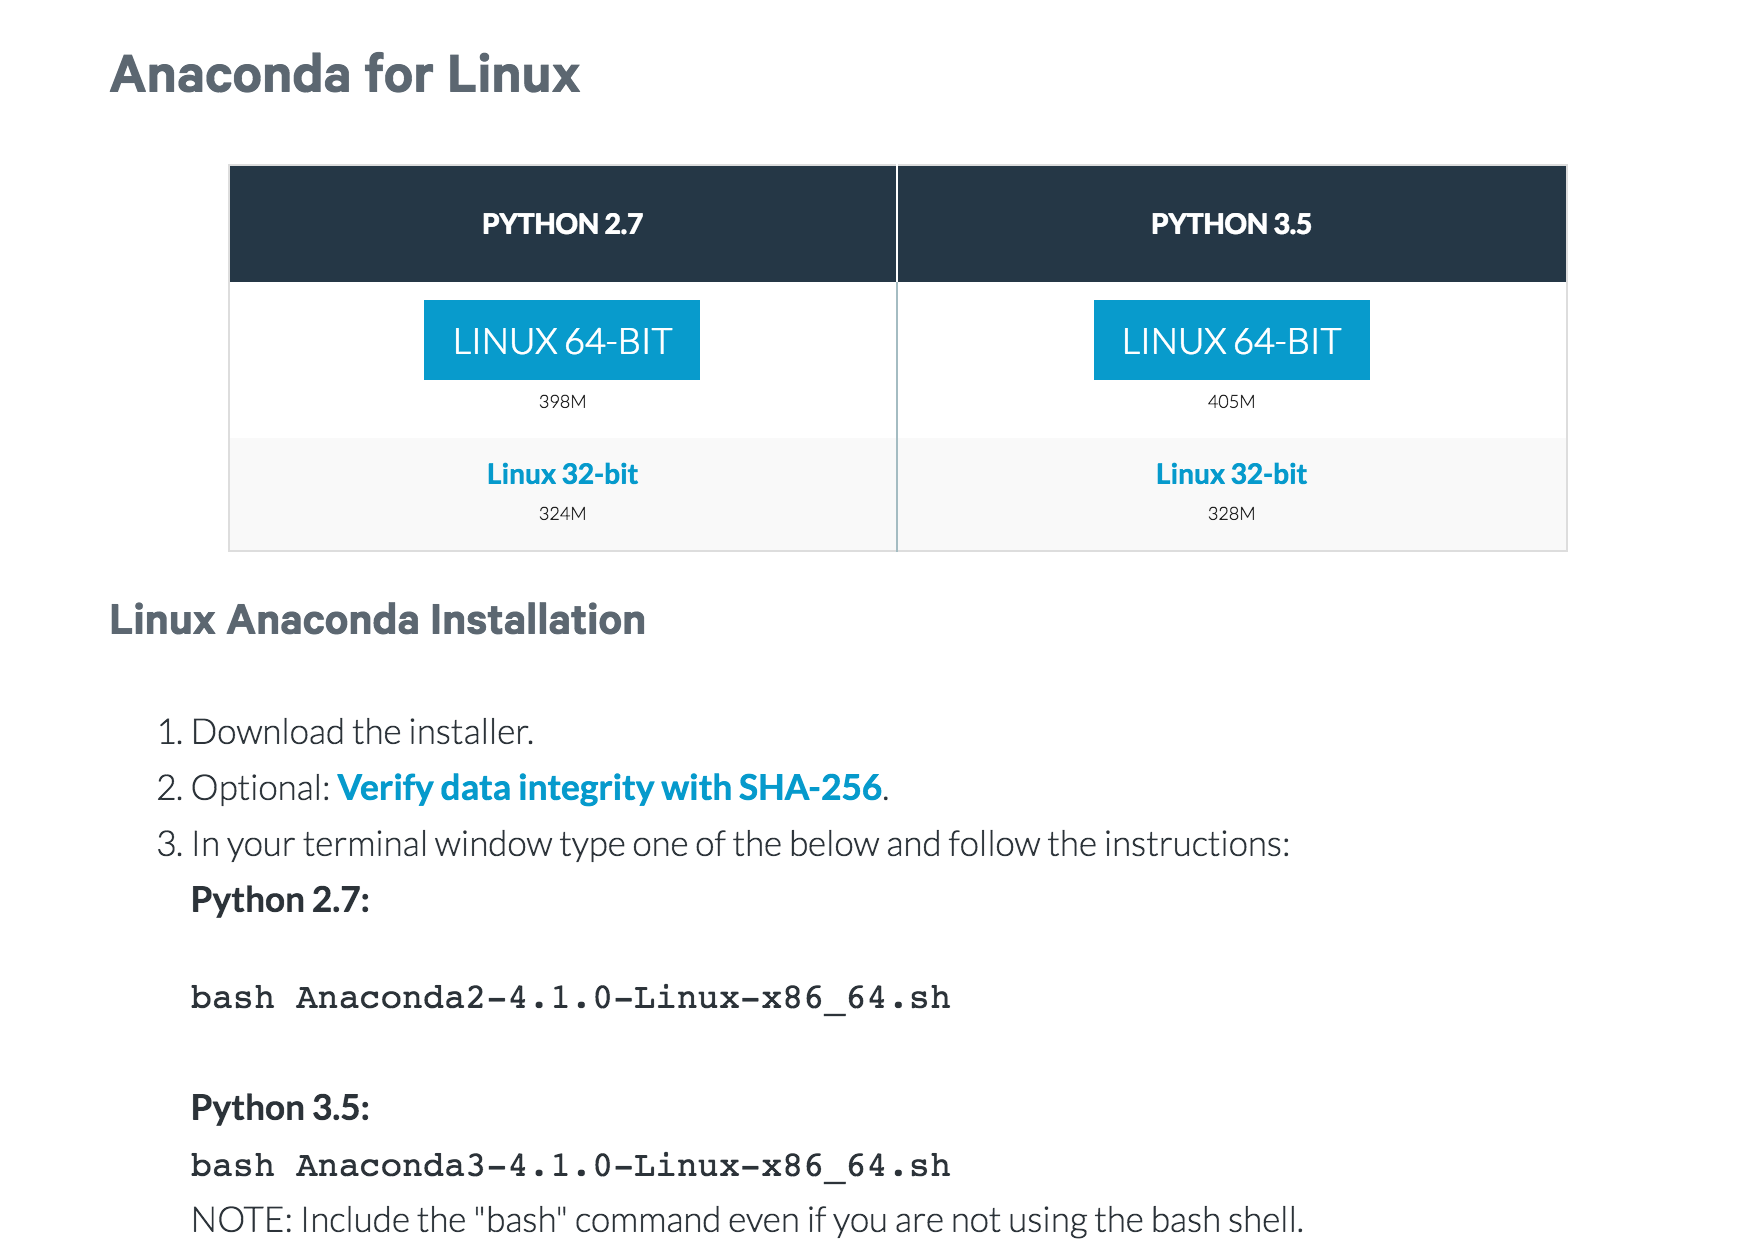
\includegraphics[scale=0.5]{linux.png}}
\end{centering}

\end{document}
